\documentclass[journal]{vgtc}                % final (journal style)
%\documentclass[review,journal]{vgtc}         % review (journal style)
%\documentclass[widereview]{vgtc}             % wide-spaced review
%\documentclass[preprint,journal]{vgtc}       % preprint (journal style)

%% Uncomment one of the lines above depending on where your paper is
%% in the conference process. ``review'' and ``widereview'' are for review
%% submission, ``preprint'' is for pre-publication, and the final version
%% doesn't use a specific qualifier.

%% Please use one of the ``review'' options in combination with the
%% assigned online id (see below) ONLY if your paper uses a double blind
%% review process. Some conferences, like IEEE Vis and InfoVis, have NOT
%% in the past.

%% Please note that the use of figures other than the optional teaser is not permitted on the first page
%% of the journal version.  Figures should begin on the second page and be
%% in CMYK or Grey scale format, otherwise, colour shifting may occur
%% during the printing process.  Papers submitted with figures other than the optional teaser on the
%% first page will be refused. Also, the teaser figure should only have the
%% width of the abstract as the template enforces it.

%% These few lines make a distinction between latex and pdflatex calls and they
%% bring in essential packages for graphics and font handling.
%% Note that due to the \DeclareGraphicsExtensions{} call it is no longer necessary
%% to provide the the path and extension of a graphics file:
%% 
\includegraphics{diamondrule} is completely sufficient.
%%
\ifpdf%                                % if we use pdflatex
  \pdfoutput=1\relax                   % create PDFs from pdfLaTeX
  \pdfcompresslevel=9                  % PDF Compression
  \pdfoptionpdfminorversion=7          % create PDF 1.7
  \ExecuteOptions{pdftex}
  \usepackage{graphicx}                % allow us to embed graphics files
  \DeclareGraphicsExtensions{.pdf,.png,.jpg,.jpeg} % for pdflatex we expect .pdf, .png, or .jpg files
\else%                                 % else we use pure latex
  \ExecuteOptions{dvips}
  \usepackage{graphicx}                % allow us to embed graphics files
  \DeclareGraphicsExtensions{.eps}     % for pure latex we expect eps files
\fi%

%% it is recomended to use ``\autoref{sec:bla}'' instead of ``Fig.~\ref{sec:bla}''
\graphicspath{{figures/}{pictures/}{images/}{./}} % where to search for the images

\usepackage{microtype}                 % use micro-typography (slightly more compact, better to read)
\PassOptionsToPackage{warn}{textcomp}  % to address font issues with \textrightarrow
\usepackage{textcomp}                  % use better special symbols
\usepackage{mathptmx}                  % use matching math font
\usepackage{times}                     % we use Times as the main font
\renewcommand*\ttdefault{txtt}         % a nicer typewriter font
\usepackage{cite}                      % needed to automatically sort the references
\usepackage{tabu}                      % only used for the table example
\usepackage{booktabs}                  % only used for the table example
%% We encourage the use of mathptmx for consistent usage of times font
%% throughout the proceedings. However, if you encounter conflicts
%% with other math-related packages, you may want to disable it.

%% In preprint mode you may define your own headline.
%\preprinttext{To appear in IEEE Transactions on Visualization and Computer Graphics.}

%% If you are submitting a paper to a conference for review with a double
%% blind reviewing process, please replace the value ``0'' below with your
%% OnlineID. Otherwise, you may safely leave it at ``0''.
\onlineid{0}

%% declare the category of your paper, only shown in review mode
\vgtccategory{Research}
%% please declare the paper type of your paper to help reviewers, only shown in review mode
%% choices:
%% * algorithm/technique
%% * application/design study
%% * evaluation
%% * system
%% * theory/model
\vgtcpapertype{please specify}

%% Paper title.
\title{Enhance Visual Analytics with Crowdsourcing through Semantic Interactions}

%% This is how authors are specified in the journal style

%% indicate IEEE Member or Student Member in form indicated below
\author{Yali Bian, Chris North}
\authorfooter{
%% insert punctuation at end of each item
\item
 Yali Bian, Chris North are with Virginia Tech. E-mail: [yali, north]@vt.eud.
}

%other entries to be set up for journal
\shortauthortitle{Biv \MakeLowercase{\textit{et al.}}: Global Illumination for Fun and Profit}
%\shortauthortitle{Firstauthor \MakeLowercase{\textit{et al.}}: Paper Title}

%% Abstract section.
\abstract{
Maing sense of large collection of document could be challenging.

How to use semantic interactions by expert to steer novice crowds (in addition to steers algorithms)
		a. input:  how to use semantic interaction as input to direct the crowd tasks
			i. can create several kinds of micro-tasks for each SI, some quick, some slow  (simulated in this paper with Tianyi data?)
				1) e.g. when expert drags 2 docs together:
					a) find entities that connect the 2 docs (quick)
					b) label semantic-level connections between the 2 docs (quick) -> text that can be used
					c) find related docs (slow)
						i) must compare to every other doc?
						ii) or use (a) and (b) to reduce the search set?  context slice?
				2) other SI ...
		b. output:  how to use crowd output in response to semantic interaction in the visualization
			i. can use crowd results in visualization (e.g. distance function for Force Directed layout)
			ii. can use crowd results in further algorithmic processing (e.g. search)
			iii. dynamic output, streaming from crowds



} % end of abstract

%% Keywords that describe your work. Will show as 'Index Terms' in journal
%% please capitalize first letter and insert punctuation after last keyword
\keywords{Visual analytics, Semantic Interaction, Crowdsourcing, Sensemaking.}

\CCScatlist{ % not used in journal version
 \CCScat{K.6.1}{Management of Computing and Information Systems}%
{Project and People Management}{Life Cycle};
 \CCScat{K.7.m}{The Computing Profession}{Miscellaneous}{Ethics}
}

%% Uncomment below to include a teaser figure.
\teaser{
  \centering
  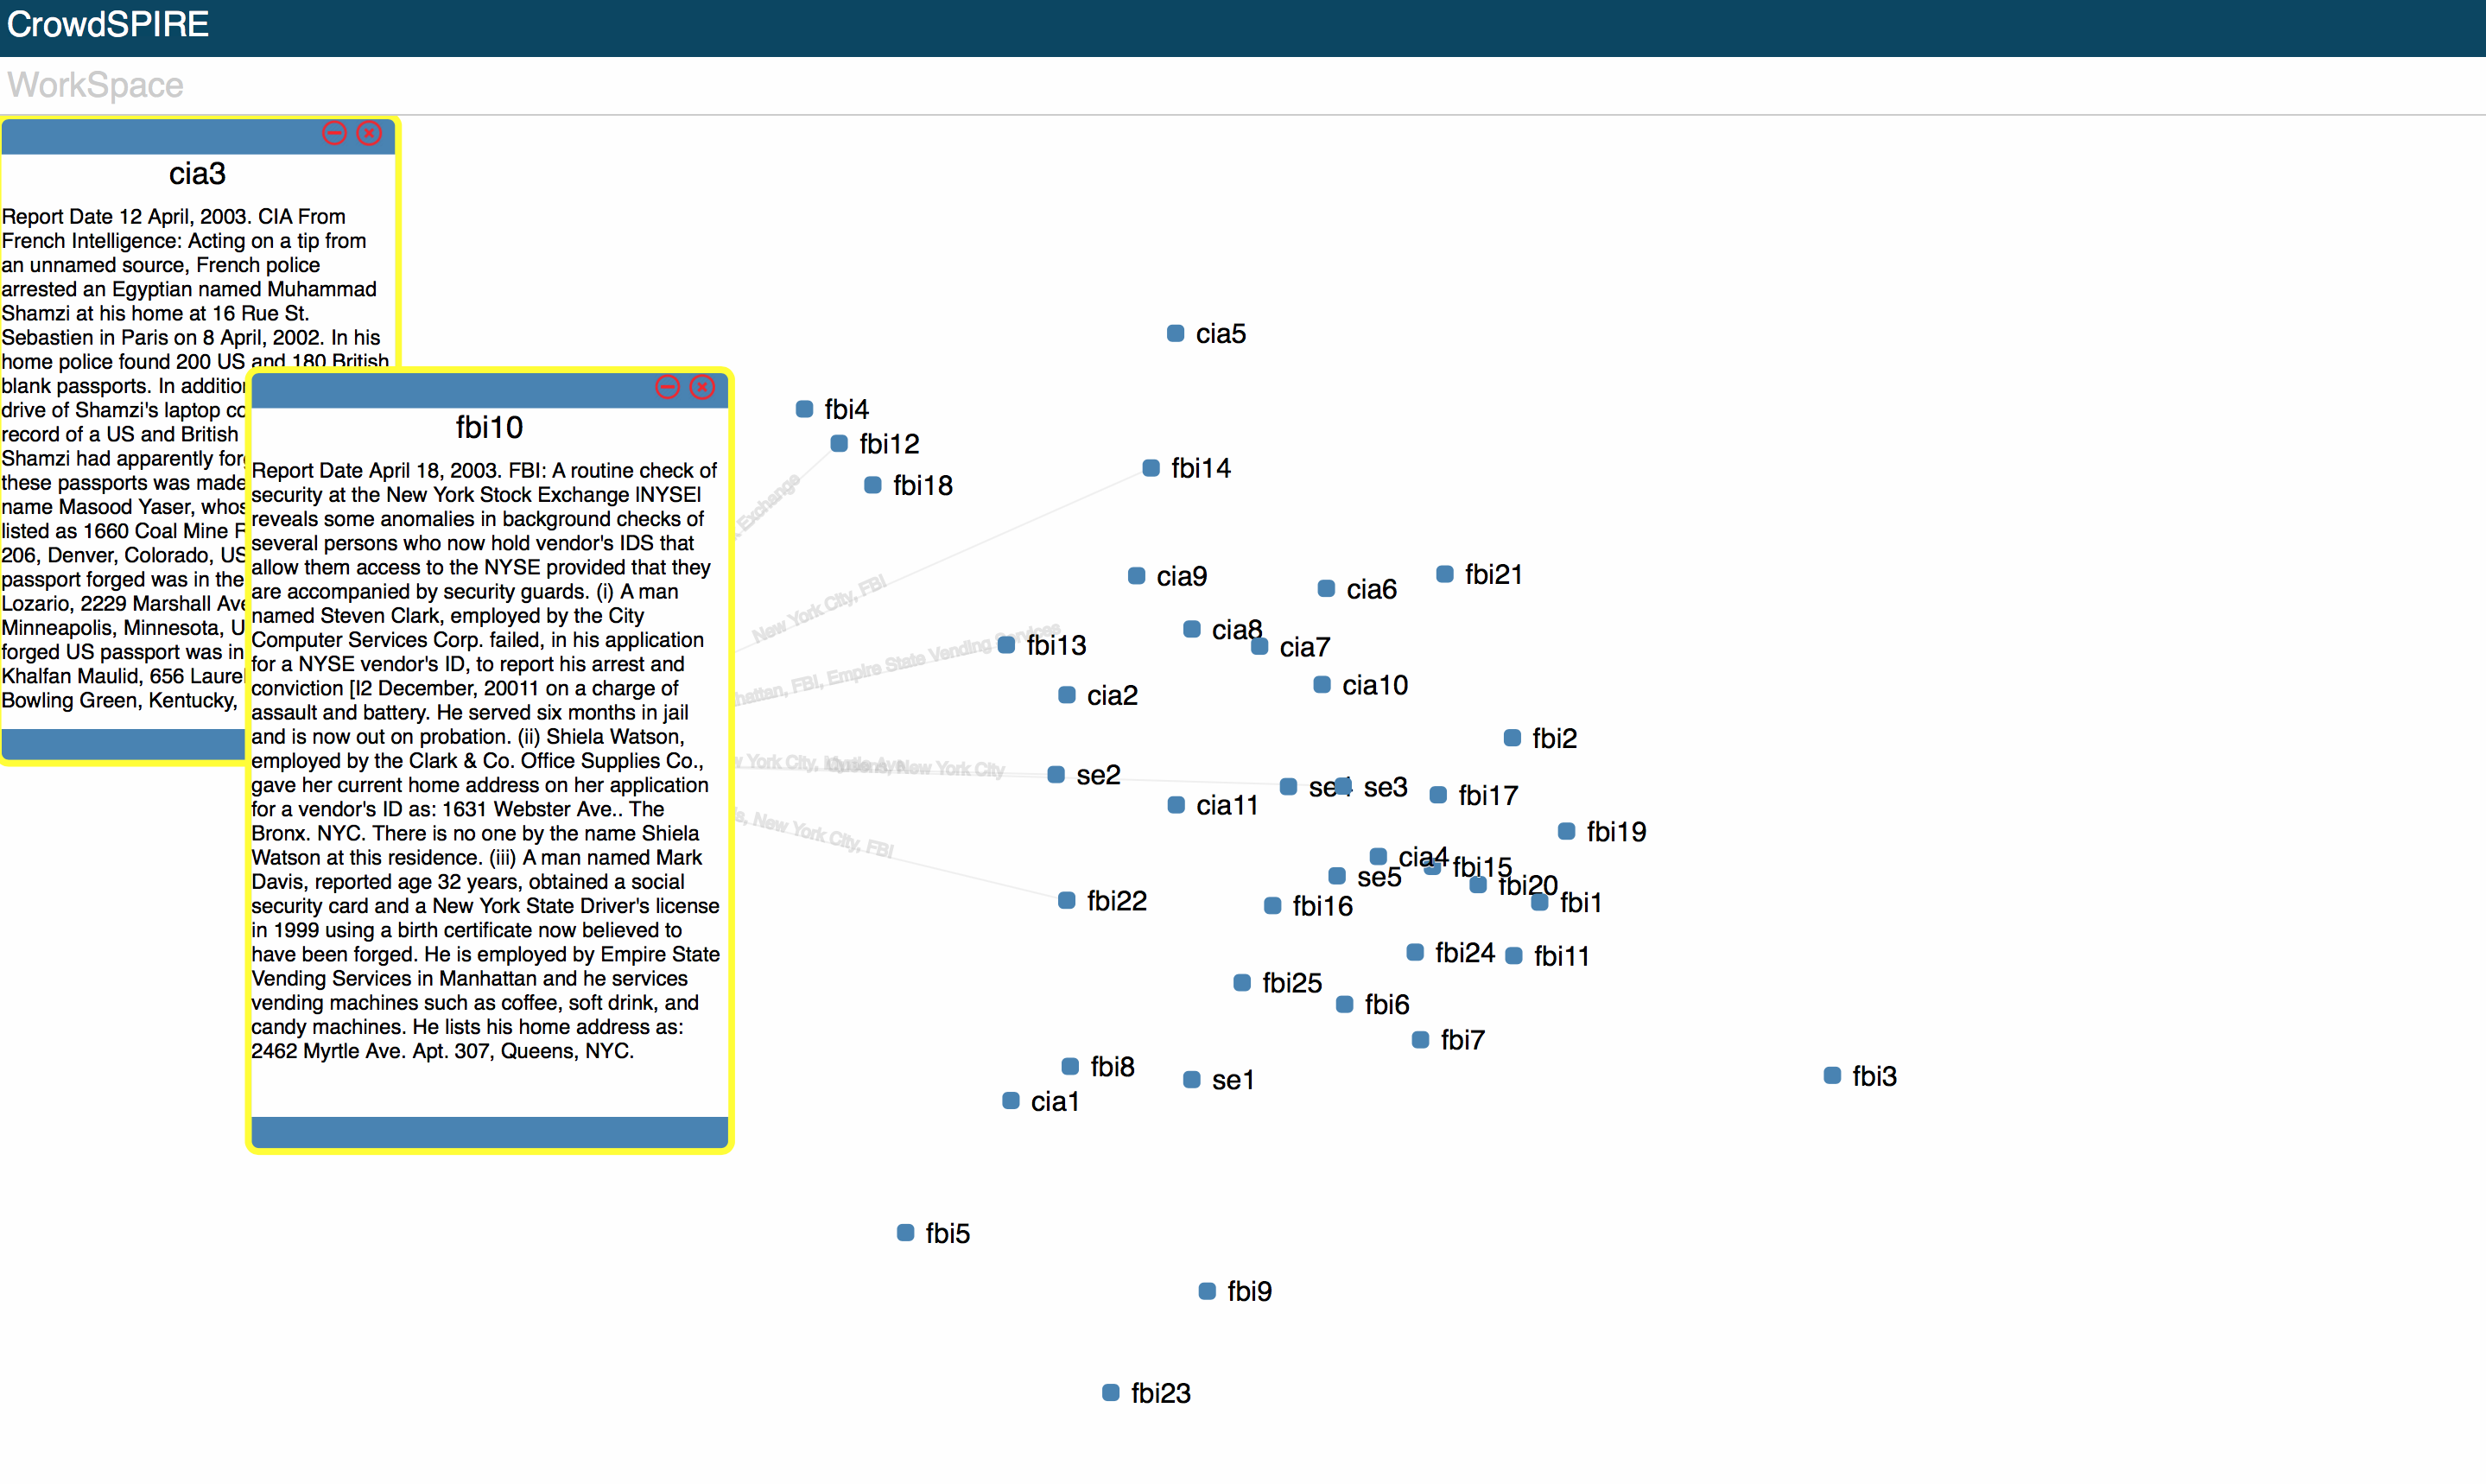
\includegraphics[width=\linewidth]{Overview}
  \caption{CrowdSPIRE: StartSPIRE based visual analytics with semantic interactions to assign crowdsourcing works}
	\label{fig:Overview}
}

%% Uncomment below to disable the manuscript note
%\renewcommand{\manuscriptnotetxt}{}

%% Copyright space is enabled by default as required by guidelines.
%% It is disabled by the 'review' option or via the following command:
% \nocopyrightspace

\vgtcinsertpkg

%%%%%%%%%%%%%%%%%%%%%%%%%%%%%%%%%%%%%%%%%%%%%%%%%%%%%%%%%%%%%%%%
%%%%%%%%%%%%%%%%%%%%%% START OF THE PAPER %%%%%%%%%%%%%%%%%%%%%%
%%%%%%%%%%%%%%%%%%%%%%%%%%%%%%%%%%%%%%%%%%%%%%%%%%%%%%%%%%%%%%%%%

\begin{document}

\firstsection{Introduction}
\maketitle
%% \section{Introduction}

We are in the midst of a data deluge that shows no signs of slowing down. Human behavior is increasingly mediated by technology, and these devices capture, store, and transmit data about their users at speeds and scales never before imagined. Documents are increasingly authored, shared, and read entirely online. Social network sites, pedometers, automobiles, and even buildings are instrumented to be sources of “big data,” and momentum is gathering to create an Internet of Things, connecting still more everyday objects to a worldwide digital network. The resulting quantities of data are astonishing. In 2008, the world generated 14.7 exabytes ($2^60$ bytes) of new information, almost three times more than just five years earlier. While some see these numbers as foreboding, others see a remarkable opportunity. If we can find ways to make sense of this big data, the possibilities for learning more about ourselves and how to improve the world we live in are almost boundless.

Yet, making sense of large amounts of data is challenging. The human mind can be immensely powerful, but it is also fundamentally constrained, in ways that have been precisely quantified, in its ability to process information [10]. Humans can only read so much text, or view so many images, or listen to so many words or sounds at a time. Thus, since the earliest days of computing, researchers and practitioners have sought to understand how computers might augment the analytical abilities of people. We have come a long way since the steam-powered calculators of Babbage and others, and today we benefit from a tremendous array of sensemaking technologies. Interactive visualization tools help us convert textual information into visual representations much faster and easier to comprehend and manipulate. Data mining and text analytics help us parse huge quantities of digitized documents to find those that are most relevant and highlight what matters about them. The emerging field of visual analytics combines these powerful approaches--information visualization and data mining--to create a new class of sensemaking tools enabling new kinds of exploration and insights.

Despite these advances, sensemaking of large datasets remains time-consuming and onerous, and existing support tools still have a long way to go. Machine learning techniques for finding, clustering, and summarizing documents can be highly effective in specialized contexts, but general purpose tools are less successful. Often, the connections that help us understand our data are more subtle than what an algorithm has been programmed to recognize. Information visualization tools amplify the cognitive abilities of their users, but many users come with limited knowledge or experience. Visual analytics overcomes some of these drawbacks by leveraging the complementary strengths of human cognition and computation, but these tools generally assist with low-level tasks, requiring significant effort on the part of users. Human sensemaking abilities remain essential and central to success.

In parallel with these developments, crowdsourcing has emerged as a promising technique for augmenting user interfaces and accomplishing tasks with which computers typically struggle. Crowdsourcing refers to online labor markets where distributed groups of people complete small amounts of work (micro-tasks), often for payment. APIs on platforms like Amazon Mechanical Turk [42] allow crowdsourced human intelligence to be applied algorithmically to complex problems and even embedded in software back-ends and user interfaces. Crowdsourcing was originally used for simple, independent tasks that leverage innate human abilities like transcribing text, identifying images, and categorizing or labeling items. More recent research investigates how complex and creative tasks, like planning a vacation, writing a news article, or shopping for a digital camera might also be crowdsourced, often with algorithms or workflows that decompose large tasks into smaller ones that can be completed in parallel.

Researchers have begun to investigate how crowdsourcing can been applied to complex sensemaking tasks, like creating a taxonomy of items or performing a bottom-up analysis of a large corpus of qualitative data. These efforts show promise for how crowds might assist an individual analyst with a difficult sensemaking problem, but differ in their emphasis on predefined data sets and goal of unsupervised task completion. One of the most significant challenges to crowdsourced sensemaking remains the ability to sustain deep or complex line of inquiry across multiple crowdworkers, who are generally novices with only a few minutes of time to commit.

In this proposal, we investigate how crowdsourcing and computational techniques can be combined to support the efforts of an individual analyst engaged in a complex sensemaking task, such as identifying a threat to national security or determining the names of people and places in a photograph. Currently, such complex tasks are beyond the capabilities of the most advanced machine learning techniques or crowdsourcing workflows, and even trained experts struggle to perform them. We propose a series of studies to understand the sensemaking process of individuals, decompose that sensemaking process into subtasks performed by crowds and automated techniques, and develop and evaluate a prototype system based on a revised sensemaking loop optimizing the complementary strengths of individuals, crowdsourcing, and computation. At the core of our approach is the novel concept of “context slices,” an innovative technique for addressing the transience of crowdworkers by using a combination of human and computational guidance to give crowd workers only the information they need to complete their assigned task. Through a series of experiments, we will show how our prototype improves upon existing best practices in general purpose tools like search engines and specialized sensemaking tools across multiple domains. This work has broad implications for making sense of big data and using crowdsourcing to perform complex tasks.



% Paper motivation
expert needs help
limits of computational methods, algorithms, cant get semantics
human crowds can help with semantics, maybe specific domain expertise?
combinatorics problem:  cant have crowd investigate all possible combinations
use expert to guide the crowd, expert has overall problem expertise
managing the crowd is onerous
how to provide expert with management capability that is usable, fits into their sensemaking process
unified interface for managing algorithms and crowds
solution = semantic interaction

\section{Related Work}
% MULTI-MODEL SEMANTIC INTERACTION
\subsection{Multi-model Semantic Interaction}
Our prior work on semantic interaction (Figure 3) was designed to enable analysts to steer computational analytical models in a usable way [8,15,17,23]. Semantic interaction shields the analysts from the low-level input parameters of the algorithms, and instead enables analysts to interact directly with the high-level outputs of the models which is where their cognition is focused. These high-level interactions are then recast into low-level inputs, through machine learning algorithms that attempt to recognize the reasoning process. For example, in text analytics, analysts can interact using Figure 3: Example of spatial text analytics their normal sensemaking actions such as reading, using our StarSpire system [8]. An expert organizing documents spatially, highlighting analyst guides the machine learning important sections, conducting searches, annotating algorithms by directly manipulating the in the margins, etc. In our StarSpire prototype [8], layout. Our vision is that the expert these actions are interpreted by the underlying interactions will also guide crowdworkers’ algorithms and applied to support the analyst by subtasks. automatically finding and organizing additional information relevant to the analyst’s thought process, integrating this visual feedback directly into the analyst’s visual spatial workspace. In our studies, we have found that this method successfully recognized analysts’ reasoning processes and relieved users from the need to organize many supporting documents or read many irrelevant documents [16]. We now recognize the opportunity to apply semantic interaction techniques to enable analysts to not only direct computational algorithms, but to also direct a large force of crowdworkers. Also, since semantic interaction recognizes opportunities for supporting subtasks and relevant information, it could also be used to support the process of generating dynamic context slices for crowdworkers’ subtasks.

\subsection{Crowdsourced synthesis and sensemaking}
Researchers have explored the value of using Figure 1: The sensemaking loop for crowdsourcing, either alone or combined with intelligence analysts described by [32]. automated approaches, to synthesize information with diverse or unknown schemas. One fruitful approach has been to blend crowdsourcing with ML algorithms. Partial clustering [19,40] and crowd kernel [35] are two such examples, but their application domain limited to imagery, and they focus on low context merges between pairs or triplets of items.

Other crowdsourcing research explores higher-context clustering. Cascade [12] produces crowdsourced taxonomies of hierarchical data sets by letting workers generate, and later select, multiple categories per item. Frenzy [11] is a web-based collaborative session organizer that elicits paper metadata by letting crowdworkers group papers into sessions using a synchronous clustering tool. We draw design inspiration from these projects, particularly the notion of integrating microtasks into a more collaborative, unstructured interface embodied in Frenzy and other forms of crowdware [41]. Our prior work builds on this research by evaluating these clustering-style interfaces compared to other interfaces and workflows.

Researchers have also studied how much context to provide crowdworkers during clustering tasks. Willet et al. [39] developed color clustering with representative sampling for reducing redundancy and capturing provenance during crowdsourced data analysis, comparing this to a pairwise “distributed clustering” approach. Andre et al. [2] compared automated clustering via TF-IDF [34], Cascade [12], and crowdsourced partial clustering adapted from Gomes et al. [19], finding that all three methods could outperform collocated experts in developing conference paper sessions. Andre et al. [1] experimented with giving crowdworkers different amounts of context prior to clustering Wikipedia barnstars. Our prior work expands on these studies by investigating a higher upper bound for context, its interaction with task structure, and synthesis across multiple documents.

Our proposed research builds on these earlier projects in significant ways. First, and most importantly, our unit of analysis is the entire sensemaking loop and ways that an individual analyst can be supported in real time by crowds or computation. We seek to augment the capabilities of these analysts, regardless of their expertise, allowing them to work faster accomplish more than they could unaided. To this end, all of our studies focus on how crowds or computation ultimately contribute to the performance of this individual. This approach is a significant departure from the majority of prior work that emphasizes unsupervised crowdsourced or computational techniques aimed at matching the performance of a motivated individual for a specific task or situation. Second, unlike most crowdsourced sensemaking projects that focus on either images or text, we investigate both domains to identify generalizable patterns and distill cross-domain design principles. Third, while prior work (including our own) establishes the importance of giving crowd workers the right amount of context, we extend this work by introducing the concept of dynamic context slices, which uses one of several methods to give each worker an amount of context customized to his or her unique task.

Real-time crowdsourcing systems have been developed to assist individuals with sensemaking tasks [5,6,26,27]. For example, VizWiz [6] is a mobile app that lets blind users capture images that sighted crowd workers can describe for them, and Chorus [27] provides a chat interface for crowd workers to help users with online search tasks like finding a nearby restaurant. We take inspiration from these systems, especially their mechanisms for recruiting and aggregating crowd work in real time, and extend them to complex sensemaking tasks where crowds are directed by mechanisms other than explicit user requests.



\section{Semantic Interactions for Crowdsourcing}

To make full use of crowdsourcing on visual analytics system, we need to find out a better way to combine crowdsourcing and visual analytics. 
Since semantic interactions is a good way to help experts to make full use of 

Visual analytics places an emphasis on the integration of data analytics into the visual data ex- ploration process.


MODEL STEERING
Model steering (sometimes referred to as computational steering) consists of the explicit or im- plicit guidance of analytic models or computation. Computational models are effective at high- lighting specific phenomena based on data characteristics in datasets. Each model comes with tradeoffs, designed and developed for specific data types, characteristics, or answers one seeks to gain from performing the computation.

Models can be steered explicitly or 


Since semantic interaction provides a link from the data in visualizations back to the analytic models that compute them. 
Semantic interaction uses the visual metaphor as a bi-direction medium through which people can analytic models can communicate and collaborate about data.
So semantic interactions could also provide as a powerful way to combinate visual analytics with crowdsourcing. 
However, crowdsourcing is different from background algorithms(Machine learning algorithms): crowdsourcing is much slower and human needed, machine computation is much faster and the scalibility
To combinate semantic interactions and crowdsourcing seamlessly. We make a new visualization pipeline as follows.




how to use semantic interactions by expert to steer novice crowds (in addition to steers algorithms). 

How to use semantic interaction as input to direct the crowd tasks.

And how to make full use of feedbacks to combined with this visual analytics system, help experts sensemaking the documents.


\subsection{Updated Visualization Pipeline}

We present an updated visualization pipeline to reflect semantic interaction for crowdsourcing. 
The initial spatialization is constructed by taking the data, or a working set of the data as determined by a relevance model, and passing it through a display layout model. 
The user then perceives the spatialization and has the option of interacting with the data within the spatial metaphor. 
All interactions are interpreted and directed to the appropriate inverted model(s). 
The inverted models then are combined, if necessary, and the new parameters are stored in the user’s high dimensional model of the data.
This high dimensional model is then coupled with the dataset to pass through the retrieval and projection portion of the loop, resulting in an updated spatialization. 
This pipeline currently assumes a single shared set of model parameters. 
Possible extensions of this pipeline include multiple user models for the data (e.g. the user believes the data should be arranged in a different manner than what the user believes should be displayed).
Not all semantic interactions will necessarily influence every model or have the same impact. 
We offer a few examples to illustrate this point. 
Highlighting a phrase in a document typically indicates its importance, while minimizing a document when space is not constricted typically indicates the unimportance of its contents.
Moving points around the display would naturally update the display layout, but would not necessarily fetch new data points for the workspace.

Furthermore, updates to the underlying models should be executed wisely. 
Updating a model that impacts the entirety of the data set will likely be a slow operation, whereas a display layout model operating on a small subset of the data can be executed much quicker. 
Therefore, it is practical to update the display layout model with each semantic interaction, but it may not be practical to do so for the information retrieval model.
Obviously, if a user explicitly queries for information, it should be returned promptly. 
Otherwise, it may be a better option to check for new potentially relevant information and/or update the underlying model every n interactions.





The overview of whole system, with input and output.

\subsection{Input}

input:  how to use semantic interaction as input to direct the crowd tasks

can create several kinds of micro-tasks for each SI, some quick, some slow  (simulated in this paper with Tianyi data?) \newline 
Drags two docs togethers
1) e.g. when expert drags 2 docs together:

a) find entities that connect the 2 docs (quick)
b) label semantic-level connections between the 2 docs (quick) -> text that can be used
c) find related docs (slow)
i) must compare to every other doc?
ii) or use (a) and (b) to reduce the search set?  context slice?\newline 


synchronous tasks

How to integrating microtasks into a more collaborative, unstructured interface embodied in Frenzy and other forms of crowdware




Open Document

Search Keywords\newline 

Clusters \newline 


\subsection{Output}

output:  how to use crowd output in response to semantic interaction in the visualization

can use crowd results in visualization (e.g. distance function for Force Directed layout)

can use crowd results in further algorithmic processing (e.g. search)

dynamic output, streaming from crowds


\section{CrowdSPIRE}

\subsection{Visual Encodings}

\subsection{Interactions}

\subsection{Related Crowdsourcing Tasks}


\section{Case Study}

Comparison of crowd-enhanced version with algorithm-only version


produces different insight?

better insight???


compare to Gold Standard Solution


beyond simple keywords, semantics similarities


compare to previous user study cluster results?

Finally we find that .

\section{Conclusion}

\acknowledgments{
The authors wish to thank A, B, C. This work was supported in part by
a grant from XYZ.}

%\bibliographystyle{abbrv}
\bibliographystyle{abbrv-doi}
%\bibliographystyle{abbrv-doi-narrow}
%\bibliographystyle{abbrv-doi-hyperref}
%\bibliographystyle{abbrv-doi-hyperref-narrow}

\bibliography{template}
\end{document}

